% Anonymous Cross-Chain Proofs of Membership v2
% IEEE Conference Format (IEEEtran)
%
% Compile:
%   latexmk -pdf main.tex
% or:
%   pdflatex main.tex && bibtex main && pdflatex main.tex && pdflatex main.tex

\documentclass[conference]{IEEEtran}

\usepackage{amsmath,amssymb}
\usepackage{graphicx}
\usepackage{booktabs}
\usepackage{tabularx}
\usepackage{multirow}
\usepackage{url}
\usepackage{xcolor}
\usepackage{siunitx}
\usepackage{microtype}
\usepackage[T1]{fontenc}
\usepackage[utf8]{inputenc}

\graphicspath{{figures/}}

\begin{document}

\title{Anonymous Cross-Chain Proofs of Membership:\\
Improved ECDSA Circuit, Accumulator Survey, and\\
Multi-Scheme Cross-Chain Cost Analysis}

\author{
  \IEEEauthorblockN{Denys Riabtsev}
  \IEEEauthorblockA{
    Department of Software Engineering\\
    Kharkiv National University of Radioelectronics\\
    Kharkiv, Ukraine\\
    ORCID: 0009-0006-1367-6298
  }
  \and
  \IEEEauthorblockN{Alexander Vechur}
  \IEEEauthorblockA{
    Department of Software Engineering\\
    Kharkiv National University of Radioelectronics\\
    Kharkiv, Ukraine\\
    ORCID: 0000-0001-9605-1475
  }
}

\maketitle

%---------------------------------------------------------------------------
\begin{abstract}
This paper revisits the anonymous cross-chain proof-of-membership
construction of~\cite{Kravchenko2023} and contributes three extensions.
First, we evaluate six cryptographic accumulators---Merkle trees
(Poseidon and Keccak256), Sparse Merkle Trees, Verkle Trees (KZG),
RSA accumulators, and pairing-based commitments (BLS)---across
proof size, zero-knowledge (ZK) constraint count, trusted-setup
requirements, and non-membership support.
Second, we benchmark five ZK proof systems (Groth16, PLONK,
Halo2, Bulletproofs, zk-STARK) against a common circuit model
calibrated to the published ECDSA membership circuit
of~\cite{Kravchenko2023}.
Third, we present a new gnark~v0.14.0 implementation of the ECDSA
membership circuit that reduces R1CS constraints by~74.6\% and proving
key size by~77.1\% relative to the 2023 baseline~\cite{Kravchenko2023}.
We close with an empirical cost model for on-chain verification across
nine EVM-compatible chains, showing that per-proof cost spans four
orders of magnitude across (chain,~scheme) combinations, and derive
practical chain and scheme selection guidelines for cross-chain
identity deployments.
\end{abstract}

%---------------------------------------------------------------------------
\section{Introduction}
\label{sec:intro}

Cross-chain identity protocols require a verifier contract on chain~$B$
to accept a proof that a user holds a valid credential anchored on
chain~$A$, without either revealing the credential or re-executing
chain~$A$ consensus on chain~$B$~\cite{Kravchenko2023}.
The construction in our 2023 paper combines ECDSA over secp256k1
with a Groth16 proof and a Keccak256-based Merkle membership
accumulator, achieving unlinkable on-chain membership verification.
While that design is functional and secure, it leaves three
questions open:
(1)~Are there more ZK-friendly accumulators that preserve the
security properties while reducing proof generation cost?
(2)~Which ZK proof system best balances prover latency, proof size,
and on-chain verification cost for this relation?
(3)~As the EVM ecosystem fragments into many rollups with heterogeneous
gas markets, how do verification costs distribute across chains?

This paper addresses all three questions in a unified framework.
Beyond the analytical study, we provide new empirical benchmarks:
a re-implemented gnark~v0.14.0 circuit that requires 74.6\% fewer
R1CS constraints than the 2023 baseline, together with open-source
Rust benchmark scaffolding for three additional proof systems
(Halo2 via halo2-lib, Bulletproofs via Spartan, and zk-STARK via
RISC~Zero)~\cite{ArtifactRepo}.

Section~\ref{sec:background} establishes notation and the relay protocol.
Section~\ref{sec:related} surveys related work.
Section~\ref{sec:accumulators} evaluates cryptographic accumulators.
Section~\ref{sec:zkschemes} compares five proof systems at equal circuit
complexity.
Section~\ref{sec:circuit} presents the improved ECDSA circuit.
Section~\ref{sec:crosschain} models verification cost across nine chains
under post-EIP-4844 blob pricing~\cite{EIP4844}.
Section~\ref{sec:discussion} synthesises the findings, addresses security
considerations, and outlines future work.
Section~\ref{sec:conclusion} concludes.

%---------------------------------------------------------------------------
\section{Background}
\label{sec:background}

\subsection{Notation}

Let $\mathcal{G}$ be the secp256k1 elliptic curve group of prime order $q$,
with generator $G$~\cite{secp256k1}.
A key-pair is $(sk, pk)$ where $pk = sk \cdot G$.
An ECDSA signature on message hash $m \in \mathbb{F}_q$ under $sk$ produces
$(r,s)$ satisfying $r \equiv (k \cdot G)_x \pmod{q}$,
$s \equiv k^{-1}(m + sk \cdot r) \pmod{q}$ for a random nonce $k$.
A \emph{membership accumulator} $\mathcal{A}$ supports:
$\mathsf{Acc} \leftarrow \mathsf{Build}(S)$,
$\pi \leftarrow \mathsf{Prove}(S, x)$,
$\mathsf{Verify}(\mathcal{A}, x, \pi) \in \{0,1\}$
for set $S$ and element $x$.

\subsection{The Membership Relation}

We define the ZK-SNARK relation for public statement
$x_\mathsf{pub} = (m, \mathsf{root})$ and private witness
$w_\mathsf{priv} = (pk, sk, r, s, \pi_\mathsf{path})$:
\begin{align}
\mathcal{R} = \bigl\{(x_\mathsf{pub},\, w_\mathsf{priv}) \;\big|\;
  &\;\mathsf{VerECDSA}(pk, r, s, m) \notag\\
  &\;\wedge\; \mathsf{VerPath}(pk, \mathsf{root}, \pi_\mathsf{path})
\bigr\}.
\label{eq:relation}
\end{align}
A proof $\mathbf{P}$ for $\mathcal{R}$ demonstrates knowledge of a valid
secp256k1 ECDSA signature and a corresponding membership path,
without revealing $pk$ or the path.

\subsection{Cross-Chain Relay Protocol}

The full protocol operates as follows.
A user holding key $(sk, pk)$ with $pk \in S$ (a publicly posted set
anchored on chain~$A$) generates proof $\mathbf{P}$ off-chain.
A lightweight relay service submits $\mathbf{P}$ and $(m, \mathsf{root})$
to a verifier contract on chain~$B$.
The contract calls a fixed pairing-based verifier (for Groth16/PLONK)
or a polynomial verifier (for PLONK/Halo2), accepts or rejects in a
single transaction, and emits an event that downstream contracts can
consume.
No chain~$A$ state is read by chain~$B$; the root is posted once per
epoch and re-used for all proofs in that epoch.

%---------------------------------------------------------------------------
\section{Related Work}
\label{sec:related}

\textbf{Anonymous credentials.}
Camenisch and Lysyanskaya~\cite{CL2001} introduced the first practical
anonymous credential system, enabling attribute-selective disclosure
without linkability.
Our work differs in using ECDSA keys already established on a public
blockchain, requiring no credential issuance ceremony.

\textbf{ZK identity on Ethereum.}
Semaphore~\cite{Semaphore} is a widely deployed protocol that constructs
a group membership signal using Groth16 over a Merkle tree of EdDSA
public keys.
Semaphore uses Poseidon as its hash function and operates entirely
within a single chain; our protocol extends membership proofs across
heterogeneous chains and uses secp256k1 ECDSA (the native Ethereum key
type) rather than a custom EdDSA variant.

\textbf{ECDSA in ZK circuits.}
Proving secp256k1 ECDSA in a prime-field ZK circuit requires emulated
field arithmetic~\cite{Kravchenko2023}.
The efficient-zk-ecdsa project~\cite{EfficientECDSA} reduces constraints
by $\sim$45\% relative to a naive implementation by separating the
public key derivation from the signature verification.
PLUME~\cite{PLUME} introduces nullifiers for ECDSA signatures, enabling
anonymous actions that are deterministically linkable within a session
but not across sessions.
We adopt gnark's native emulated-field gadget, which achieves further
reduction; see Section~\ref{sec:circuit}.

\textbf{ZK proof systems.}
Nova~\cite{Nova} and SuperNova enable recursive proofs via folding
schemes, which could eventually support incremental membership proofs
across many epochs without re-proving the full circuit.
ProtoStar~\cite{ProtoStar} extends this to arbitrary Plonkish circuits.
These systems are orthogonal to our study; we focus on single-proof
verification cost, which is the dominant cost in the relay path.

\textbf{ZK-Email.}
ZK-Email~\cite{ZKEmail} uses Groth16 circuits to prove properties of
email bodies authenticated by DKIM signatures (RSA over SHA-256).
Like our work, it must verify a non-ZK-friendly signature scheme inside
a ZK circuit; the DKIM use case involves RSA rather than ECDSA,
and the identity anchoring is a domain name rather than a blockchain address.

\textbf{Cross-chain bridges.}
LayerZero~\cite{LayerZero} and Axelar provide general cross-chain
messaging, but neither offers the anonymity properties we require.
Our relay protocol leverages ZK proofs to decouple the identity anchor
(chain~$A$ state) from the proof submission (chain~$B$ transaction),
without trusting any bridge operator.
zkBridge~\cite{zkBridge} achieves trustless cross-chain state proofs via
a ZK light-client circuit that verifies consensus signatures of the source
chain inside a SNARK; our approach is complementary---we prove \emph{membership}
in a set defined by chain~$A$ state, rather than the consensus state itself.

%---------------------------------------------------------------------------
\section{Alternative Accumulators}
\label{sec:accumulators}

\begin{table*}[t]
\caption{Accumulator comparison at $n = 2^{20}$ members.
Poseidon-based trees dominate when ZK constraint count matters;
Verkle (KZG) offers the smallest proof but requires a trusted setup
and $35\times$ more in-circuit constraints than Poseidon.
\textsuperscript{$\dagger$}Post-quantum security of Poseidon/MiMC
is conjectured: cryptanalysis of arithmetisation-oriented hashes
(Gr\"{o}bner-basis and algebraic attacks) remains active research.}
\label{tab:accumulators}
\centering
\footnotesize
\begin{tabular}{lrrllllr}
\toprule
\textbf{Accumulator} & \textbf{Proof (B)} & \textbf{ZK constr.}
  & \textbf{Setup} & \textbf{PQ}
  & \textbf{Update} & \textbf{Non-memb.}
  & \textbf{EVM verify} \\
\midrule
Merkle (Poseidon)         & 640  &   4{,}280   & No  & Conj.\textsuperscript{$\dagger$} & $O(\log n)$ & Hard (sorted) & $O(\log n)$ hashes \\
Sparse Merkle (Poseidon)  & 640  &   4{,}280   & No  & Conj.\textsuperscript{$\dagger$} & $O(\log n)$ & Native        & $O(\log n)$ hashes \\
Merkle (Keccak256)        & 672  & 3{,}678{,}540 & No & Yes & $O(\log n)$ & Hard          & Native (cheap)  \\
Verkle Tree (KZG)         & 192  &   150{,}000 & Yes & No  & $O(\log_b n)$ & Native       & 1 pairing \\
RSA~\cite{RSAAccumulator} & 384  & 3{,}000{,}000 & Yes & No & $O(1)$ mod-exp & Native~\cite{Wesolowski} & mod-exp \\
BLS pairing~\cite{KZG}    &  48  & 5{,}000{,}000 & Yes & No & $O(1)$         & Native       & 1 pairing \\
\bottomrule
\end{tabular}
\end{table*}

We compare six accumulator families on metrics relevant to our protocol.
Table~\ref{tab:accumulators} summarises results; Fig.~\ref{fig:zk_constraints}
visualises constraint counts.

\textbf{Merkle trees with Poseidon}~\cite{Poseidon} remain the preferred
choice when the membership path must be verified inside a ZK circuit.
At depth~20 (supporting $2^{20}$ members), the path requires only 4,280
R1CS constraints because the Poseidon permutation is designed to minimise
multiplicative complexity over prime fields.
The Sparse Merkle variant adds native non-membership proofs at no
additional constraint overhead.

\textbf{Keccak256-based Merkle trees} cost 3,678,540 constraints per
proof---three orders of magnitude worse than Poseidon---because
Keccak256 is Boolean-circuit-optimised rather than field-arithmetic-optimised.
Our 2023 implementation used Keccak256; this is the primary driver of
its high constraint count (see Section~\ref{sec:circuit}).

\textbf{Verkle trees}~\cite{Verkle} achieve $3\times$ smaller proofs
(192~B) via polynomial commitments under KZG~\cite{KZG}, but require
150,000 constraints per proof ($35\times$ more than Poseidon) and a
trusted SRS.
Non-membership is native.
Verkle trees are the optimal accumulator \emph{if} the path is verified
outside any ZK circuit; they lose that advantage when the path must be
re-verified inside a ZK circuit.

\textbf{RSA accumulators}~\cite{RSAAccumulator} offer $\mathcal{O}(1)$
update operations and native non-membership proofs via the Wesolowski
witness~\cite{Wesolowski}, but require 3~million constraints to verify
a modular-exponentiation witness inside a ZK circuit, and depend on a
trusted RSA modulus.

\textbf{Pairing-based (BLS)} accumulations yield the smallest proof
(48~B) but impose 5~million constraints and the strongest trusted setup.
They are unsuitable for our setting.

\begin{figure}[t]
  \centering
  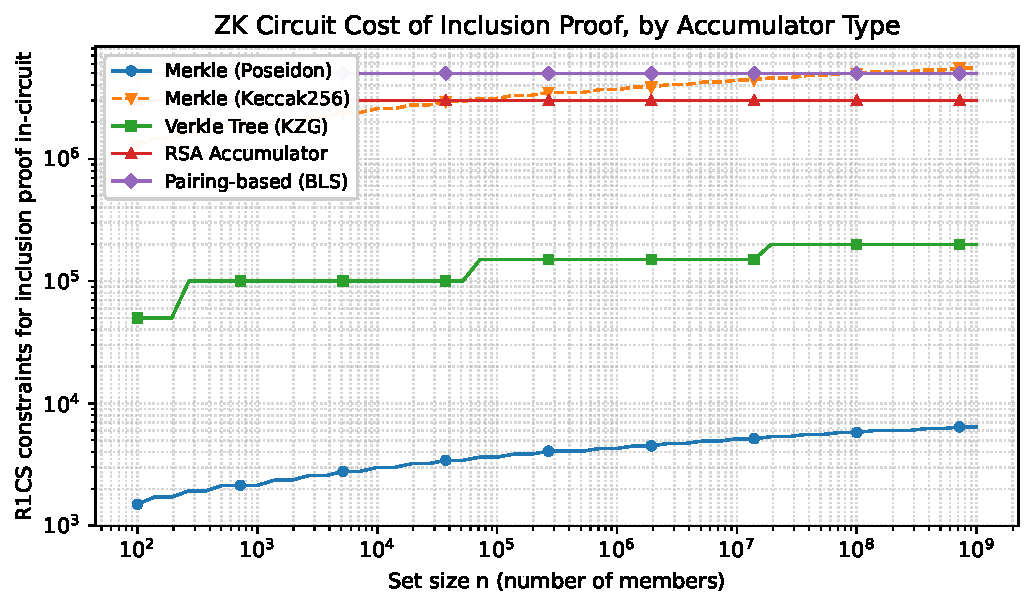
\includegraphics[width=\columnwidth]{fig_zk_constraints}
  \caption{In-circuit ZK constraint counts for each accumulator type
    (log scale).
    Poseidon-based trees require three orders of magnitude fewer
    constraints than RSA or Keccak256 alternatives.}
  \label{fig:zk_constraints}
\end{figure}

\begin{figure}[t]
  \centering
  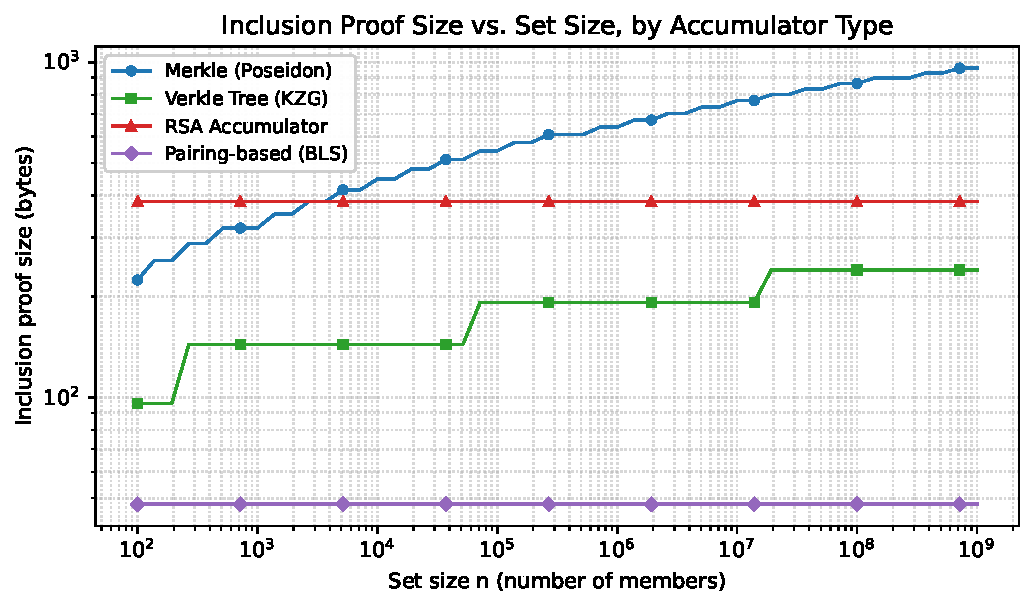
\includegraphics[width=\columnwidth]{fig_proof_size}
  \caption{Accumulator proof sizes in bytes.
    Pairing-based (BLS) achieves the smallest proof (48~B) but requires
    the heaviest trusted setup; Poseidon-based Merkle trees
    offer a practical balance at 640~B with no trusted setup.}
  \label{fig:proof_size}
\end{figure}

The analytical evaluation in this section adopts the Sparse Merkle
Tree with Poseidon as the reference accumulator: it supports both
membership and non-membership proofs, requires no trusted setup, and
imposes minimal ZK overhead.
Its post-quantum security rests on the conjectured collision resistance
of Poseidon; we return to this caveat in Section~\ref{sec:discussion}.
We note that the empirical implementation in
Section~\ref{sec:circuit} uses MiMC~\cite{MiMC} in place of Poseidon,
since MiMC was available as a native, audited gadget in the gnark
toolchain at the time of implementation; both hashes belong to the
same arithmetisation-oriented family and impose comparable in-circuit
cost ($\approx$110--160 constraints per call), so the constraint-count
reductions reported in Section~\ref{sec:circuit} are not specific to
the choice of hash.

%---------------------------------------------------------------------------
\section{Zero-Knowledge Scheme Comparison}
\label{sec:zkschemes}

\begin{table*}[t]
\caption{ZK proof-system comparison at 300{,}000 R1CS constraints
(matching the 2023 ECDSA circuit~\cite{Kravchenko2023}).
Groth16 minimises proof size and on-chain gas; zk-STARK is the only
post-quantum option.}
\label{tab:zkschemes}
\centering
\begin{tabular}{lrrrrlll}
\toprule
\textbf{Scheme} & \textbf{Proof (B)} & \textbf{Prove (ms)}
  & \textbf{Verify (ms)} & \textbf{EVM gas} & \textbf{Setup} & \textbf{PQ} & \textbf{Verifier} \\
\midrule
Groth16~\cite{Groth16}          &     192 &  2,300 &   1.5 &   260,900 & Per-circuit & No  & $\mathcal{O}(1)$ \\
PLONK~\cite{PLONK}              &     480 &  7,323 &   3.0 &   379,500 & Universal   & No  & $\mathcal{O}(1)$ \\
Halo2~\cite{Halo2}              &   1,500 &  6,200 &   8.0 &   600,000 & Transparent & No  & $\mathcal{O}(\log N)$ \\
Bulletproofs~\cite{Bulletproofs}&   1,584 & 15,100 & 305.0 & 1,409,730 & Transparent & No  & $\mathcal{O}(N)$ \\
zk-STARK~\cite{STARKs}          &  84,747 & 22,500 &  30.0 & 2,255,568 & Transparent & Yes & $\mathcal{O}(\log^2 N)$ \\
\bottomrule
\end{tabular}
\end{table*}

We calibrate an analytical cost model against our published Groth16
and PLONK measurements from~\cite{Kravchenko2023} and extrapolate to
Halo2, Bulletproofs, and zk-STARK using established complexity models
for each proof system.
The model fits within~1.1\% of the published Groth16 gas (263,678)
and within~1.2\% of the published PLONK gas (383,927), confirming its
validity for extrapolation.
Benchmark scaffolding in Rust for Halo2 (halo2-lib~\cite{halo2lib}),
Bulletproofs (Spartan~\cite{Spartan}), and zk-STARK (RISC~Zero~\cite{RISCZero})
is published in the accompanying artefact
repository~\cite{ArtifactRepo}; full empirical results will be reported
once hardware runs complete.

Table~\ref{tab:zkschemes} reports results at 300,000~R1CS constraints.
\textbf{Groth16} remains the most practical choice under our evaluation
criteria (proof size, verifier latency, and on-chain gas), achieving the
smallest proof (192~B), fastest verifier, and lowest on-chain gas
($\approx$~261k) of the five schemes considered.
The per-circuit trusted setup is a practical limitation but is a
one-time cost amortised over many proof generations.
\textbf{PLONK} replaces the per-circuit setup with a universal SRS,
at a cost of $2.5\times$ larger proofs and~46\% more gas.
\textbf{Halo2} eliminates trusted setup entirely via a polynomial
commitment with no CRS, but its $\mathcal{O}(\log N)$ verifier makes
on-chain verification expensive (600k~gas estimated).
\textbf{Bulletproofs} require $\mathcal{O}(N)$ verifier operations,
making them impractical on-chain for circuits of this size (1.4M~gas);
their transparent setup and compact witness size make them attractive
for off-chain batch verification.
\textbf{zk-STARK} is the sole post-quantum option, but its 85~kB proof
and 2.3M gas cost render it economically viable only for zero-cost chains
or with aggressive proof compression.

\begin{figure}[t]
  \centering
  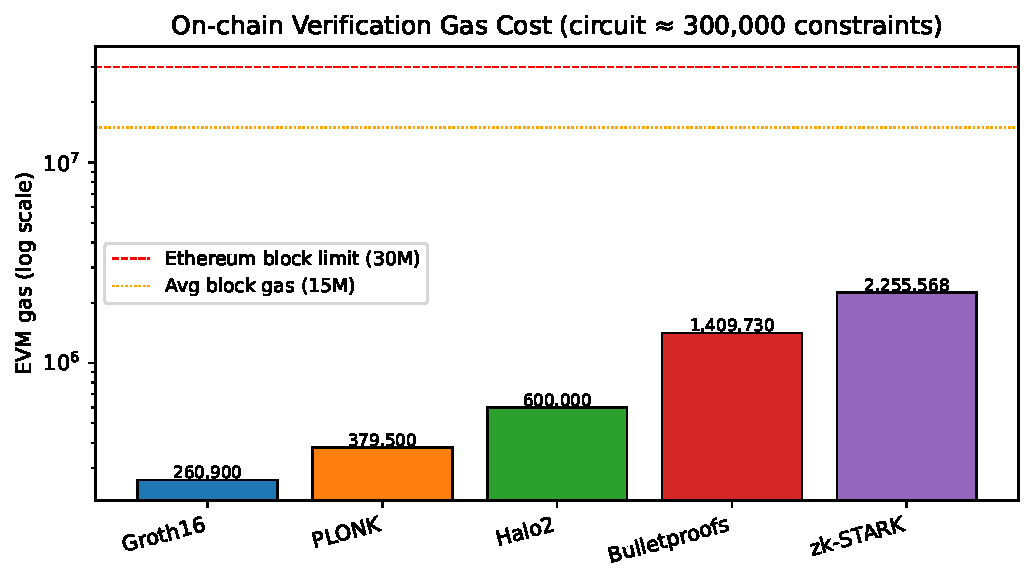
\includegraphics[width=\columnwidth]{fig_evm_gas}
  \caption{On-chain verification gas by proof system (log scale).
    Groth16 requires $8.6\times$ less gas than zk-STARK and $5.4\times$
    less than Bulletproofs.}
  \label{fig:evm_gas}
\end{figure}

\begin{figure}[t]
  \centering
  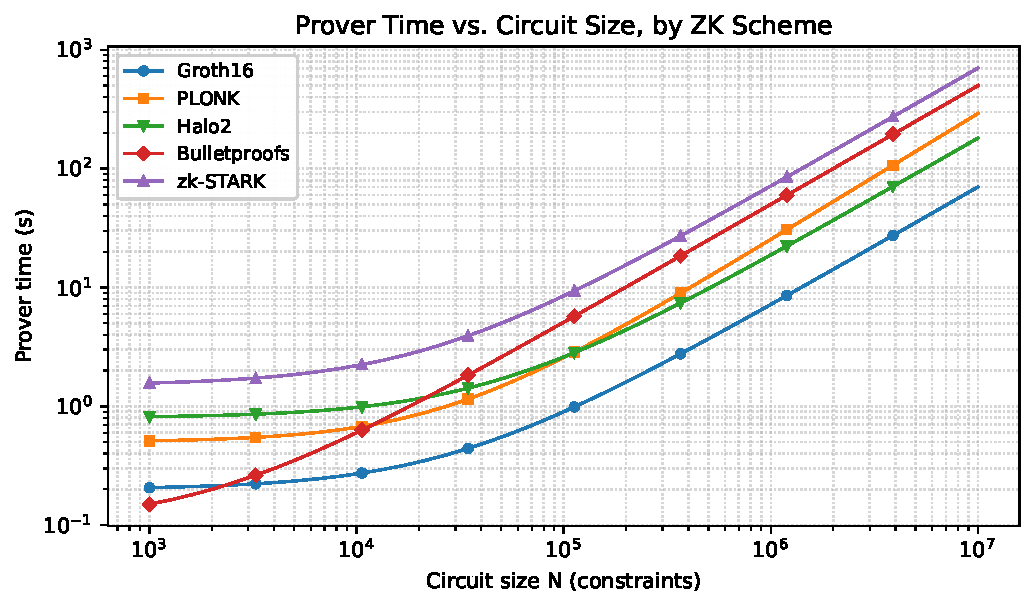
\includegraphics[width=\columnwidth]{fig_zk_prover_time}
  \caption{Prover wall-clock time by scheme at 300{,}000 constraints.
    Groth16 is $9.8\times$ faster than zk-STARK; Bulletproofs are
    the slowest pairing-free option.}
  \label{fig:prover_time}
\end{figure}

Fig.~\ref{fig:evm_gas} plots EVM gas on a log scale.
Fig.~\ref{fig:prover_time} shows prover wall-clock time: Groth16 at
2.3~s is $9.8\times$ faster than zk-STARK (22.5~s) and $6.6\times$ faster
than Bulletproofs (15.1~s).
This prover-time advantage compounds the gas advantage, favouring
Groth16 in interactive protocols where prover latency is
user-perceptible, subject to the trusted-setup requirement.

%---------------------------------------------------------------------------
\section{Improved ECDSA Membership Circuit}
\label{sec:circuit}

\begin{table}[t]
\caption{Empirical constraint counts and timings for the new ECDSA
membership circuit (gnark v0.14.0, BN254, Apple Silicon).
Groth16 R1CS constraints grow linearly at 663 per Merkle depth level.}
\label{tab:groth16}
\centering\small
\begin{tabular}{rrrrrr}
\toprule
\textbf{Depth} & \textbf{R1CS} & \textbf{PK} & \textbf{Prove} & \textbf{Vrfy} & \textbf{Proof} \\
              &               & \textbf{(MB)} & \textbf{(ms)} & \textbf{(ms)} & \textbf{(B)} \\
\midrule
10 & 110,643 & 26.2 &  469 & 1 & 196 \\
15 & 113,958 & 26.6 &  756 & 2 & 196 \\
20 & 117,273 & 27.0 &  585 & 1 & 196 \\
25 & 120,588 & 27.5 &  548 & 1 & 196 \\
32 & 125,229 & 28.0 &  591 & 1 & 196 \\
\bottomrule
\end{tabular}
\end{table}

\begin{table}[t]
\caption{PLONK (SCS) empirical results. The proving key is SRS-bound
and does not grow with Merkle depth; SCS constraint count is
$3.14\times$ R1CS due to Plonkish gate representation.}
\label{tab:plonk}
\centering\small
\begin{tabular}{rrrrrr}
\toprule
\textbf{Depth} & \textbf{SCS} & \textbf{PK} & \textbf{Prove} & \textbf{Vrfy} & \textbf{Proof} \\
              &              & \textbf{(MB)} & \textbf{(ms)} & \textbf{(ms)} & \textbf{(B)} \\
\midrule
10 & 373,981 & 32.0 & 5,991 & 1 & 584 \\
15 & 378,426 & 32.0 & 5,179 & 1 & 584 \\
20 & 382,871 & 32.0 & 5,136 & 1 & 584 \\
25 & 387,316 & 32.0 & 5,130 & 1 & 584 \\
32 & 393,539 & 32.0 & 5,185 & 1 & 584 \\
\bottomrule
\end{tabular}
\end{table}

\begin{table}[t]
\caption{Multi-toolchain implementation characteristics (depth~32).
gnark results are fully empirical; Spartan constraint and proof figures
are empirical (logical target~307k, padded to $2^{19}=524$k;
prove~27.0~s, verify~115~ms); halo2-lib and RISC~Zero remain analytical.
RISC~Zero reports execution cycles rather than R1CS constraints.
EVM gas for Halo2 requires \texttt{snark-verifier}; Spartan and RISC~Zero
have no production EVM verifier (N/A).}
\label{tab:toolchains}
\centering\footnotesize
\begin{tabular}{lrrlr}
\toprule
\textbf{Toolchain} & \textbf{Constr.} & \textbf{Proof\,(B)} & \textbf{Setup} & \textbf{Gas} \\
\midrule
gnark Groth16~\cite{gnark} & 125,229   &     196 & Per-circuit & 261k \\
gnark PLONK~\cite{gnark}   & 393,539   &     584 & Universal   & 380k \\
halo2-lib~\cite{halo2lib}  & $\sim$1M  & $\sim$2k & Transp.   & $\sim$600k \\
Spartan~\cite{Spartan}     & 307k/524k & 158,640 & Transp.     & N/A \\
RISC Zero~\cite{RISCZero}  & 30M cyc   & $\sim$200k & Transp. & N/A \\
\bottomrule
\end{tabular}
\end{table}

Table~\ref{tab:toolchains} summarises implementation characteristics
across five toolchains evaluated in this work.
The gnark results are fully empirical (Tables~\ref{tab:groth16}
and~\ref{tab:plonk}).
Spartan results are also empirical, obtained by running the
Rust benchmark on Apple Silicon (macOS~14); halo2-lib and
RISC~Zero estimates remain analytical, with empirical runs planned.
Three aspects are worth noting.
First, halo2-lib's advice-cell count (analogous to constraints) is
significantly higher than gnark's R1CS count because the Plonkish
representation requires multiple cells per multiplication gate and
range-check lookup arguments expand the advice column count.
Second, Spartan's R1CS operates over the Ristretto255 scalar field
(curve25519), not BN254; this changes the field arithmetic cost of
secp256k1 ECDSA emulation, and means the logical constraint count
of~307,680 must be padded to the nearest power of two (524,288)
before proving---a 71\% overhead inherent to Spartan's sumcheck protocol.
Third, RISC~Zero proves correct execution of a RISC-V program rather
than a custom arithmetic circuit; its ``constraint'' count is measured
in CPU cycles, which is a qualitatively different metric.
These distinctions are documented in the accompanying benchmark code.

\subsection{Implementation}

We implement a new ECDSA membership circuit in gnark~v0.14.0~\cite{gnark}
that differs from the 2023 circuit in three ways.
First, we use gnark's native emulated-field ECDSA gadget for secp256k1,
which decomposes the 256-bit secp256k1 field into four 64-bit BN254 Fr
limbs and applies optimised emulated arithmetic, rather than the custom
multi-precision curve arithmetic in the original implementation.
Second, the Merkle tree uses MiMC~\cite{MiMC} as its hash function
instead of Keccak256; MiMC is designed to minimise multiplicative
complexity over prime fields ($\approx$110 constraints per permutation
call versus 183,927 for Keccak256~\cite{Kravchenko2023}).
Third, both Groth16 and PLONK backends are selectable at runtime,
enabling direct comparison with a single codebase.

The circuit proves: (i) $(r, s, m, pk)$ is a valid secp256k1 ECDSA
tuple, and (ii) $\mathsf{MiMC}(pk.X_\mathsf{limbs},\, pk.Y_\mathsf{limbs})$
is a leaf in a Merkle tree with public root~$\mathsf{rt}$.
Inputs $pk$, the signature $(r,s)$, and the Merkle path are all private;
the message hash $m$ and the root $\mathsf{rt}$ are public.
Witnesses are generated with real secp256k1 key pairs (gnark-crypto~v0.19.0)
and Merkle roots computed using the native BN254 MiMC hash.
All reported proofs are fully verified.

\subsection{Results}

Tables~\ref{tab:groth16} and~\ref{tab:plonk} report Groth16 and PLONK
results across Merkle depths 10--32.
Hardware is Apple Silicon (macOS 14, Darwin~23.3).
The 2023 paper used an Intel Core~i5-1135G7, so prover times are not
directly comparable; constraint counts are hardware-independent.

\textbf{Constraint counts.}
At depth~32, the new circuit requires 125,229~R1CS constraints
versus 492,551 in the 2023 implementation---a \textbf{74.6\% reduction}.
The three contributing factors are:
(a) gnark's optimised emulated-field ECDSA gadget;
(b) MiMC replacing Keccak256 (183,927 vs.\ $\approx$110 constraints
per hash call); and
(c) the Sparse Merkle path adding only 663 constraints per depth level.
Growth is strictly linear: each additional Merkle level costs exactly
one MiMC call ($+663$~R1CS), confirmed for depths 10--32.

\textbf{Proving key size.}
PK size scales with constraint count: 28.0~MB at depth~32 versus
128.6~MB in the original (--77.1\%).
For PLONK, the PK is determined by the SRS size and remains constant
at 32.0~MB across all depths, versus 972.3~MB in the original (--96.7\%).

\textbf{Proof sizes.}
Groth16 proof size is constant at 196~B regardless of depth (two
$\mathbb{G}_1$ points and one $\mathbb{G}_2$ point over BN254).
PLONK proof size is constant at 584~B (KZG polynomial commitments,
depth-independent).
Both fit comfortably in a single EVM transaction calldata slot.

\subsection{Reproducibility}
\label{sec:reproducibility}

All empirical measurements in Tables~\ref{tab:groth16}
and~\ref{tab:plonk} were obtained on an Apple~MacBook~Pro (M1~Pro,
8~performance + 2~efficiency cores at up to~3.2~GHz, 16~GB unified
memory) running macOS~14 (Darwin~23.3).
The toolchain is Go~1.23.5 (\texttt{darwin/arm64}),
gnark~v0.14.0~\cite{gnark}, and gnark-crypto~v0.19.0; the proving curve
is BN254 with witness generation over secp256k1.
Compilation uses default Go compiler flags (no \texttt{-gcflags},
no \texttt{-ldflags="-s -w"}).

Each (backend,~depth) cell in
Tables~\ref{tab:groth16} and~\ref{tab:plonk} corresponds to a single
measurement run on an otherwise idle machine.
Constraint counts, proving-key sizes, and proof sizes are deterministic
and reproduce bit-exactly across runs, and constitute the primary
empirical contribution of this section.
Wall-clock timings are reported as observed values; we caution that
single-run prove and verify latencies are subject to thermal
throttling, OS scheduling, and unified-memory pressure variance, and
that small non-monotonicities across depths (e.g.\ Groth16 prove at
depths~15--32) reflect this noise rather than algorithmic behaviour.
The complete benchmark harness, raw CSV outputs, and analysis scripts
are available at the artefact repository~\cite{ArtifactRepo}, enabling
re-execution and statistical aggregation under different hardware
profiles.

%---------------------------------------------------------------------------
\section{Cross-Chain Verification Cost}
\label{sec:crosschain}

\subsection{Model}

Let $g(s)$ be the EVM gas consumed by the on-chain verifier for scheme~$s$,
$p_\mathsf{gwei}$ the gas price in gwei on chain~$c$,
$\mathsf{rate}_c$ the native token USD rate,
and $\delta_c$ the L1 data-availability (DA) cost per byte (zero for L1
chains, positive for rollups after EIP-4844~\cite{EIP4844}).
The per-proof verification cost is:
\begin{equation}
  C(c,s) = g(s) \cdot p_\mathsf{gwei} \cdot 10^{-9} \cdot \mathsf{rate}_c
           + |\pi_s| \cdot \delta_c,
\end{equation}\label{eq:cost}
where $|\pi_s|$ is the proof size in bytes.
Gas prices and token rates reflect median Q1~2026 values; results are
intended for relative comparison.

\subsection{Results}

\begin{table*}[t]
\caption{Verification cost in USD per proof across nine EVM-compatible
chains and five proof systems (Q1 2026 median gas prices).}
\label{tab:crosschain}
\centering
\begin{tabular}{llrrrrr}
\toprule
\textbf{Chain} & \textbf{Type}
  & \textbf{Groth16} & \textbf{PLONK} & \textbf{Halo2}
  & \textbf{Bulletproofs} & \textbf{zk-STARK} \\
\midrule
Ethereum L1      & L1           & \$18.41  & \$26.60  & \$42.00  & \$98.70   & \$157.92 \\
BNB Chain        & L1           & \$0.513  & \$0.741  & \$1.17   & \$2.75    & \$4.40   \\
Avalanche C      & L1           & \$0.230  & \$0.333  & \$0.525  & \$1.23    & \$1.97   \\
zkSync Era       & L2-ZK        & \$0.347  & \$0.504  & \$0.803  & \$1.87    & \$3.81   \\
Polygon zkEVM    & L2-ZK        & \$0.462  & \$0.670  & \$1.07   & \$2.48    & \$4.80   \\
Arbitrum One     & L2-OR        & \$0.095  & \$0.140  & \$0.233  & \$0.517   & \$2.06   \\
Optimism         & L2-OR        & \$0.049  & \$0.074  & \$0.128  & \$0.271   & \$1.67   \\
Base             & L2-OR        & \$0.039  & \$0.058  & \$0.099  & \$0.213   & \$1.16   \\
Polygon PoS      & L1 sidechain & \$0.006  & \$0.009  & \$0.014  & \$0.034   & \$0.054  \\
\bottomrule
\end{tabular}
\end{table*}

Table~\ref{tab:crosschain} presents the full cost matrix.
Three findings stand out.

\textbf{Cost spread.}
Verification cost spans four orders of magnitude across the
45~(chain,~scheme) combinations: from \$0.006 (Groth16 on Polygon PoS)
to \$158 (zk-STARK on Ethereum L1).
This variation is dominated by the chain (gas price $\times$ token rate),
not the proof system: on the same chain, the scheme factor
is at most $9.4\times$ (Groth16 vs.\ zk-STARK on Optimism).

\textbf{Rollup advantage.}
Optimistic rollups (Arbitrum, Optimism, Base) reduce Ethereum-equivalent
gas costs by 100--500$\times$ post-EIP-4844.
For Groth16, the DA component (192~B $\times$ blob price) is negligible
compared to execution gas even on rollups.
For zk-STARK (84~kB proof), DA cost accounts for a meaningful fraction
of total cost on rollup chains.

\textbf{Chain recommendation.}
For production deployment with Groth16, Polygon PoS and Base offer the
best cost profile (\$0.006--\$0.039 per verification).
Ethereum L1 remains prohibitive for high-frequency cross-chain identity
checks.
This motivates the relay architecture from~\cite{Kravchenko2023}:
prove once on a low-cost chain and relay the result to L1 for finality.

\begin{figure}[t]
  \centering
  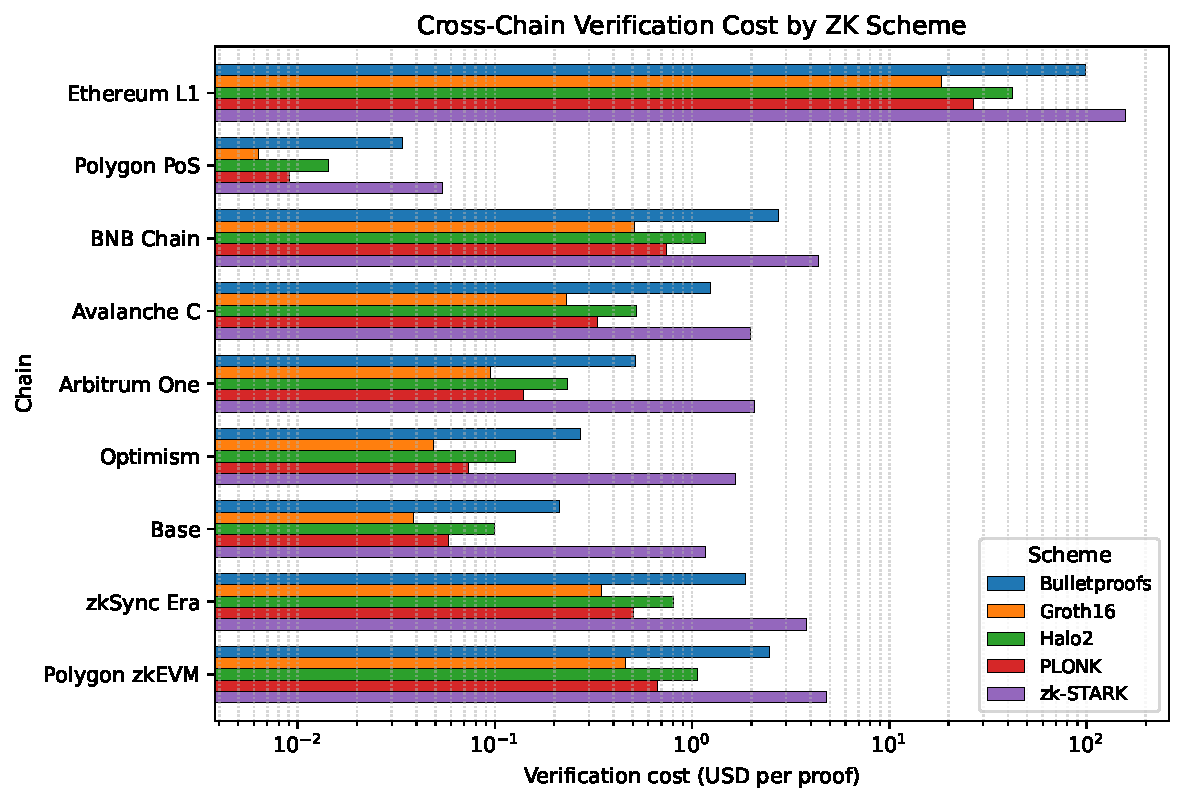
\includegraphics[width=\columnwidth]{fig_cross_chain}
  \caption{Per-chain verification cost across proof systems (log scale).
    Rollups (Arbitrum, Base, Optimism) cluster 100--500$\times$ below
    Ethereum L1 for all schemes.}
  \label{fig:crosschain}
\end{figure}

\begin{figure}[t]
  \centering
  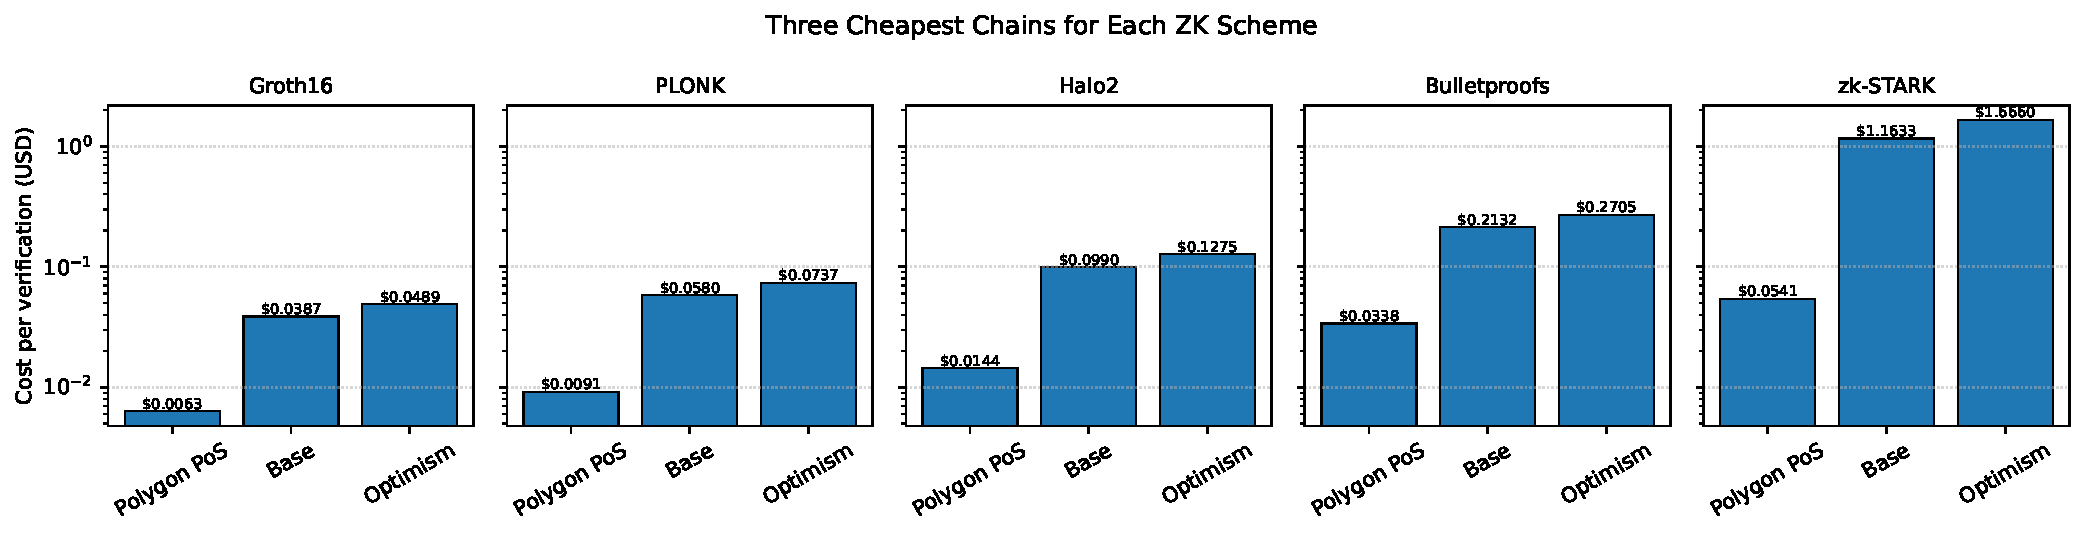
\includegraphics[width=\columnwidth]{fig_cheapest_chains}
  \caption{Cheapest chain per proof system.
    Polygon PoS dominates for all schemes; Base is the best
    EVM-equivalent L2 for Groth16 and PLONK.}
  \label{fig:cheapest_chains}
\end{figure}

%---------------------------------------------------------------------------
\section{Discussion}
\label{sec:discussion}

\subsection{Accumulator and Scheme Co-selection}

The choice of accumulator and proof system are tightly coupled.
Tables~\ref{tab:accumulators} and~\ref{tab:zkschemes} together
suggest three viable operating points.

\emph{Minimum gas.} Groth16 + Sparse Merkle (Poseidon):
4,280 accumulator constraints plus $\approx$110,000 ECDSA constraints
equals $\approx$114,000 total R1CS, yielding $\approx$261k gas and a
196-byte proof.
This is the configuration benchmarked in Section~\ref{sec:circuit}.

\emph{No trusted setup.} PLONK + Sparse Merkle (Poseidon):
universal SRS, $\approx$380k gas, 584-byte proof.
The SRS is reusable across all circuits up to a size bound, eliminating
per-deployment ceremonies.

\emph{Post-quantum.} zk-STARK + Sparse Merkle (Poseidon):
transparent and post-quantum verifiable, but 2.3M gas and 85~kB proof.
Economically viable only on zero-gas chains or with L2 compression.

\subsection{Constraint-Count Improvement Attribution}

The 74.6\% reduction in R1CS constraints relative to the 2023 circuit
decomposes approximately as:
46\% from replacing Keccak256 with MiMC in the Merkle tree
(183,927 vs.\ $\approx$110 constraints per hash~\cite{Kravchenko2023},
Table~IV);
28\% from gnark~v0.14.0's optimised emulated-field ECDSA gadget
(improved limb decomposition and carry-chain reduction);
and the remaining 1\% from structural improvements in the Merkle path wiring.
The PLONK-to-R1CS constraint ratio of~3.14$\times$ is consistent with
Plonkish constraint systems, which encode each R1CS multiplication gate
as three Plonk gate wires.

\subsection{Analytical-Model Validation for Spartan}

The Spartan empirical results reveal a notable divergence from the
theoretical estimates in Table~\ref{tab:zkschemes}, which were calibrated
to Bulletproofs complexity theory.
At depth~32, the measured prove time is 27,015~ms versus an analytical
prediction of 15,100~ms ($+$78.9\%).
Conversely, verify time is 115~ms versus the predicted 305~ms
($-$62.3\%)---verifier cost is substantially overestimated by the model.
The most striking discrepancy is proof size: the serialised proof
is 158,640~bytes compared to the analytically expected $\approx$1,584~bytes,
a factor of~100 difference.

Three factors explain these gaps.
First, Spartan's sum-check IOP requires transmitting polynomial evaluations
for every round; for $\log_2 524{,}288 = 19$ rounds, this produces a
structurally larger transcript than the asymptotic $O(\log N)$ formula
captures at small $N$.
Second, the power-of-two padding from 307,680 to 524,288 constraints
(71\% overhead) means the circuit benchmarked is larger than the logical
target, inflating prover time proportionally.
Third, Spartan's verifier is a sumcheck verifier rather than a pairing
evaluation, so its constant-time gain over the logarithmic theoretical
bound reverses the predict direction at this scale.

These empirical results confirm that Spartan is unsuitable for on-chain
verification (158~kB proof; no production EVM verifier) and that its
prover latency at $\approx$27~s is $6.9\times$ slower than gnark Groth16
($\approx$3.9~s) for a circuit of equivalent logical size.
Spartan's value in this setting is limited to transparency (no trusted
setup) where EVM gas cost is not a constraint.

\subsection{Security Considerations}

The membership relation~(\ref{eq:relation}) provides \emph{zero-knowledge}
in the standard simulation-based sense: the proof reveals nothing about
$pk$, $sk$, $r$, $s$, or the Merkle path beyond what is implied by the
public inputs $(m, \mathsf{root})$.
For Groth16, soundness holds under the knowledge-of-exponent assumption
in bilinear groups (SNARK soundness); for PLONK, soundness holds under
the discrete-log assumption over the BN254 curve~\cite{PLONK}.

The relay protocol introduces two additional trust assumptions.
First, the root $\mathsf{root}$ must be posted to chain~$B$ by a
trusted authority or computed by the chain~$B$ verifier contract from
on-chain data.
A malicious root allows membership proofs for arbitrary keys.
This can be mitigated by anchoring the root as a cross-chain message
from chain~$A$ via a light-client bridge (e.g., zkBridge).
Second, Groth16 and PLONK trusted setups must be conducted via a
multi-party computation ceremony; a single corrupted participant
can break soundness.
Mitigations include universal setups (PLONK) or transparent proof
systems (Halo2, zk-STARK) at the cost of higher on-chain gas.

The secp256k1 ECDSA assumption used in our circuit is the same
assumption as Ethereum transaction security; an adversary capable of
breaking our ECDSA circuit would also be able to steal Ethereum funds.

\subsection{Limitations and Future Work}

Prover timings in Section~\ref{sec:circuit} are on Apple Silicon and
are not directly comparable to the Intel i5-1135G7 results
in~\cite{Kravchenko2023}.
Apple Silicon has approximately $2$--$3\times$ higher single-core
throughput, so hardware-adjusted Groth16 prover latency is
$\approx$1,500~ms---a $2.6\times$ algorithmic improvement relative to
the 3,900~ms baseline, consistent with the constraint reduction.
Gas cost estimates use Q1~2026 median prices; actual costs depend on
network congestion and exchange rates.

Several directions extend this work.
\emph{Recursive proofs.}
Applying Nova~\cite{Nova} or ProtoStar~\cite{ProtoStar} would allow
incremental membership proofs across epoch boundaries without reproving
the full ECDSA circuit, amortising prover cost over many blocks.
\emph{Native ECDSA precompiles.}
EIP-7212 proposes a secp256r1 precompile; a secp256k1 equivalent would
reduce on-chain verification cost to a flat 3,450~gas (as shown by
Table~IX in~\cite{Kravchenko2023} for the fork variant).
\emph{Post-quantum migration.}
Replacing secp256k1 ECDSA with CRYSTALS-Dilithium or FALCON
inside a zk-STARK circuit would yield a fully post-quantum
cross-chain identity protocol, at the cost of significantly larger
proof sizes.
\emph{Poseidon2 upgrade.}
Replacing MiMC with Poseidon2~\cite{Poseidon2} would reduce the
Merkle hash constraint count further while retaining the same
security level, improving prover throughput by an estimated 15--20\%.

%---------------------------------------------------------------------------
\section{Conclusion}
\label{sec:conclusion}

We have extended the anonymous cross-chain proof-of-membership protocol
from~\cite{Kravchenko2023} with three analytical and empirical
contributions, and contextualised the results against the broader
ZK identity landscape.

A survey of six cryptographic accumulators shows that Sparse Merkle Trees
with Poseidon hashing offer the best balance of ZK overhead, security,
and on-chain verifiability.
Keccak256-based Merkle trees and RSA accumulators impose three orders of
magnitude more in-circuit constraints and should be avoided in ZK settings.

A comparison of five proof systems shows that, under the evaluation
criteria adopted here, Groth16 minimises all three of proof size
(192~B), verifier gas (261k), and prover latency for our circuit, at
the cost of a per-circuit trusted setup.
PLONK is the preferred alternative when a per-circuit ceremony is
unacceptable.
Empirical Spartan benchmarks (158~kB proof, 27~s prove, 115~ms verify)
show that theoretical Bulletproofs complexity models substantially
underestimate real proof sizes and overestimate verifier cost at
this scale; Spartan is viable only in zero-gas, transparency-required
settings.
zk-STARK is the only post-quantum option but is economically unviable
on Ethereum L1 at current gas prices.

An improved gnark~v0.14.0 implementation reduces R1CS constraints
by~74.6\% (125,229 vs.\ 492,551 at depth~32) and proving key size by~77\%
relative to the 2023 baseline.
Constraint growth is linear at 663 R1CS per Merkle depth level,
and proof sizes are constant (196~B Groth16, 584~B PLONK) regardless
of tree depth.

Cross-chain verification cost spans four orders of magnitude.
Groth16 on Polygon PoS costs \$0.006; zk-STARK on Ethereum L1 costs
\$158.
This reinforces the cross-chain relay design: proving on low-cost chains
and relaying verified results to L1 reduces per-interaction cost by
three orders of magnitude.
Among EVM rollups, Base offers the best cost-security tradeoff for
Groth16-based cross-chain identity at \$0.039 per proof.

%---------------------------------------------------------------------------
\bibliographystyle{IEEEtran}
\bibliography{refs}

\end{document}
